\section{Obiettivi e aspettative}

\begin{figure}[!h] 
  \centering 
  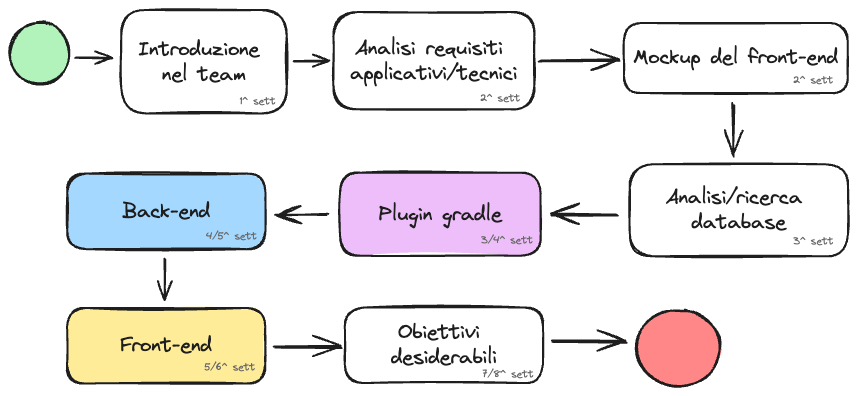
\includegraphics[width=1\columnwidth]{workflow-stage} 
  \caption{Sequenza temporale delle attività scritte nel piano di lavoro.}
  \label{fig:workflow-stage}
\end{figure}

L'identificazione degli obiettivi e delle aspettative è un passo fondamentale per la definizione di un progetto di \stage.
In questo contesto, gli obiettivi rappresentano le funzionalità che il sistema deve implementare, mentre le aspettative
sono le caratteristiche che il sistema deve possedere.\\
Gli obiettivi e le aspettative del progetto di \stage{} sono stati definiti in collaborazione con il \textit{tutor} aziendale, 
tramite il piano di lavoro.
Esso è stato redatto prima dell'inizio dello \stage, e ha rappresentato un punto di riferimento per la valutazione
delle attività svolte durante il periodo di \stage.\\
All'interno del piano di lavoro erano presenti obiettivi obbligatori e obiettivi desiderabili.
Gli obiettivi avevano un codice identificativo, e una descrizione.\\ 
Il codice identificativo era composto da una lettera che rappresentava la tipologia di obiettivo, e da un numero progressivo.
Il progressivo ha permesso l'ordinamento, non casuale, degli obiettivi. \\
La pianificazione settimanale scritta nel piano di lavoro, riportata in figura \ref*{fig:workflow-stage}, è stata una vera e propria 
guida per lo svolgimento delle attività, ed 
ha permesso di rispettare le scadenze, raggiungendo gli obiettivi prefissati in ordine di priorità, portando quelli desiderabili
a termine solo se il tempo lo avrebbe permesso.\\

Nel piano di lavoro gli obiettivi non erano molto dettagliati (tabella \ref*{tab:obiettivi-obbligatori} e tabella \ref*{tab:obiettivi-desiderabili}), questo ci ha permesso di avere una certa flessibilità durante lo svolgimento
delle attività, e di poter cambiare gli obiettivi in corso d'opera, se necessario.\\

\begin{table}[!h]
  \caption{Obiettivi obbligatori}
  \label{tab:obiettivi-obbligatori}
\begin{tabularx}{\textwidth}{lX}
   \textbf{Identificativo}&\textbf{Descrizione}\\ 
    \hline O01&Analisi dell'attuale infrastruttura\\
    \hline O02&Analisi requisiti applicativi e tecnici e \textit{mockup} del \textit{frontend}\\
    \hline O03&Identificazione del db a grafo più adeguato al progetto\\
    \hline O04&Implementazione della struttura di \textit{database}\\
    \hline O05&Implementazione di un \textit{plugin} Gradle per la raccolta delle informazioni\\
    \hline O06&Invocazione da \textit{jenkins}\\
    \hline O07&Implementazione dei servizi \textit{backend} per l'interrogazione del sistema\\
    \hline O08&Implementazione del \textit{frontend} per rendere possibile l'interrogazione\\
    \hline 
\end{tabularx}
\end{table}

  \begin{table}[!h]
    \caption{Obiettivi desiderabili}
    \label{tab:obiettivi-desiderabili}
    \begin{tabularx}{\textwidth}{lX}
    \textbf{Identificativo}&\textbf{Descrizione}\\ 
    \hline D01&Possibilità di visualizzare i risultati in forma grafica (grafo) e non solo tabellari\\
    \hline D02&Integrazione con \textit{repository} remoti al fine di verificare nuove versioni delle dipendenze\\
    \hline D03&Integrazione con \textit{repository} remoti al fine di identificare vulnerabilità sulle dipendenze utilizzate\\
    \hline D04&Login con LDAP aziendale\\  
    \hline
  \end{tabularx}
  \end{table}
